\documentclass[]{article}
\usepackage[top=2.5cm, bottom=2.5cm, left=3cm, right=3cm]{geometry}
\usepackage{amsmath,amssymb,amsfonts,latexsym,textcomp} %paquetes matematicos
\usepackage{array,multirow,booktabs,tabulary} %tablas y arrays
\usepackage{graphicx}   
\usepackage{caption,float,subfigure} %float=figuras flotantes.
\usepackage{verbatim}  %texto raw 
\usepackage[ampersand]{easylist} %http://en.wikibooks.org/wiki/LaTeX/List_Structures#Easylist_package 
\usepackage{subfigure}
\usepackage{color}
\usepackage[usenames,dvipsnames,svgnames,table,x11names]{xcolor} 

%font for mathcal using mathalfa
\usepackage[cal=cm]{mathalfa}  %https://tex.stackexchange.com/questions/58098/what-are-all-the-font-styles-i-can-use-in-math-mode


%---- Usar otros fonts + símbolo \degree -----------------------------------
\newcommand*{\myfont}{\fontfamily{lmtt}\selectfont}
\DeclareTextFontCommand{\textmyfont}{\myfont}	
\usepackage{gensymb} 

%---- Code highlighting con Listings ---------------------------------------
\usepackage{listings}	
\definecolor{mygreen}{rgb}{0.5,0.6,0.5}
\definecolor{mygray}{rgb}{0.5,0.5,0.5}
\definecolor{mymauve}{rgb}{0.58,0,0.82}
\definecolor{mygray2}{rgb}{0.9764, 0.9764, 0.9762}
%---- Config listings ------------------------------------------------------
\lstset{ %
	backgroundcolor=\color{mygray2},	% background color
	basicstyle=\footnotesize\ttfamily,	% tamaño de las letras y tipo de letra
	breaklines=true,	% corte de linea (line breaking)solo en espacio blanco
	captionpos=t,		% posicion del caption b,t,n (top,bottom,none)
	commentstyle=\color{ForestGreen},	% estilo del comentario
	%escapeinside={\%*}{*},	% si se desea agregar codigo Latex dentro el codigo debe ser %*codigo latex*
	frame=single,	% agrega marco al codigo
	frameround=tttt,	% redondear el marco
	keepspaces=true,	% mantiene los espacios en el texto, util para mantener la indentacion del codigo (uso posible en columns=flexible)
	keywordstyle=\color{blue},	% estilo de los keywords
	stringstyle=\color{mymauve},	% estilo del string
	numbers=left,	% donde poner los numeros de linea, (none, left, right)
	numbersep=5pt,	% cuan lejos los numeros de linea estan del codigo
	xleftmargin=0pt,	% margen izquierdo
	showspaces=false,	% muestra espacios de codigo en todas partes usando el caracter barra baja "_", sobreescribe el comando 'showstringspaces'
	showstringspaces=false,	% muestra espacios solo en los strings
	tabsize=2,	% tabulacion por defecto =2
	title=\lstname	% muestra el nombre de lo archivos incluidos con \lstinputlisting; tambien se puede tratar con caption en vez de title
}	
%---- Config personalizada del caption -------------------------------------
\DeclareCaptionFont{white}{ \color{white} }
\DeclareCaptionFormat{listing}{
	\colorbox[cmyk]{0.43, 0.35, 0.35, 0.01 }{
		\parbox{0.96\linewidth}{\hspace{15pt}#1#2#3}
	}
}
\captionsetup[lstlisting]{ format=listing, 
	labelfont=white, 
	textfont=white, 
	singlelinecheck=false, 
	margin=0pt, 
	font={bf,footnotesize} }
%---- Caracteres especiales ------------------------------------------------	
% Por defecto, listings no soporta inputec para mostrar los acentos y caracteres especiales.
% para manejar utf8 se debe enlistar los caracteres segun:
\lstset{literate=
	{á}{{\'a}}1 {é}{{\'e}}1 {í}{{\'i}}1 {ó}{{\'o}}1 {ú}{{\'u}}1
	{Á}{{\'A}}1 {É}{{\'E}}1 {Í}{{\'I}}1 {Ó}{{\'O}}1 {Ú}{{\'U}}1
	{à}{{\`a}}1 {è}{{\`e}}1 {ì}{{\`i}}1 {ò}{{\`o}}1 {ù}{{\`u}}1
	{À}{{\`A}}1 {È}{{\'E}}1 {Ì}{{\`I}}1 {Ò}{{\`O}}1 {Ù}{{\`U}}1
	{ä}{{\"a}}1 {ë}{{\"e}}1 {ï}{{\"i}}1 {ö}{{\"o}}1 {ü}{{\"u}}1
	{Ä}{{\"A}}1 {Ë}{{\"E}}1 {Ï}{{\"I}}1 {Ö}{{\"O}}1 {Ü}{{\"U}}1
	{â}{{\^a}}1 {ê}{{\^e}}1 {î}{{\^i}}1 {ô}{{\^o}}1 {û}{{\^u}}1
	{Â}{{\^A}}1 {Ê}{{\^E}}1 {Î}{{\^I}}1 {Ô}{{\^O}}1 {Û}{{\^U}}1
	{œ}{{\oe}}1 {Œ}{{\OE}}1 {æ}{{\ae}}1 {Æ}{{\AE}}1 {ß}{{\ss}}1
	{ç}{{\c c}}1 {Ç}{{\c C}}1 {ø}{{\o}}1 {å}{{\r a}}1 {Å}{{\r A}}1
	{ñ}{{\~n}}1 {£}{{\pounds}}1 {°}{{\degree}}1
}		
%---- Macro de inclusión de documentos con listings ------------------------
% [2]=numero de argumentos, #1=argumento 1, #2=argumento 2
\newcommand{\includecode}[2]{\lstinputlisting[language=#1, caption=#2, label=#2]{#2}}			



% --- Fig and table command -----------------------------------------------
%\newcommand{\figref}[1]{\figurename~\ref{#1}}
\newcommand{\figref}[1]{Fig.~\ref{#1}}
\newcommand{\tabref}[1]{Table~\ref{#1}}
\newcommand{\algref}[1]{Algorithm~\ref{#1}}


%=============================================================================================
%opening
\title{EE4323 Industrial Control Systems\\ 
		Homework Assignment 1\\
		\underline{Dynamics model of a DC motor with gear train}}
\author{Paulo R. Loma Marconi}
\date{May 4, 2017}

\begin{document}
\maketitle

The objective is to model the dynamics of a DC servo motor with gear train, \figref{fig:DCmotor}, and to deduce two equilibrium points.

\begin{figure}[!ht]
	\centering
	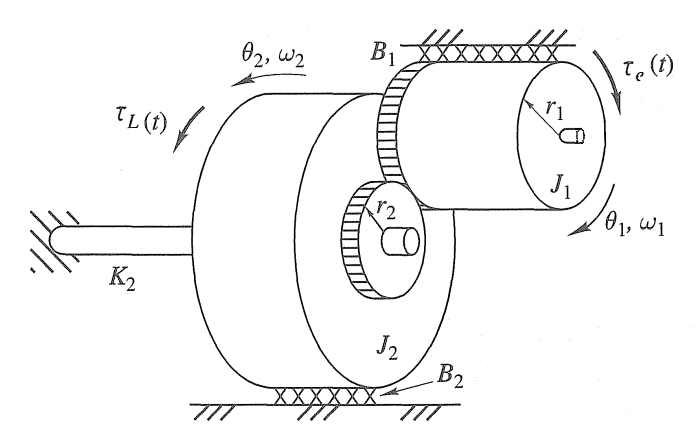
\includegraphics[width=0.5\linewidth]{DCmotor}
	\caption{DC servo motor with gear train.}
	\label{fig:DCmotor}
\end{figure}

\section{Free-body diagram analysis}
The system can be decomposed in two sections: a rotational mechanical, and an electronmechanical. The rotational mechanical can be derived as follows,

\begin{figure}[H]
	\centering
	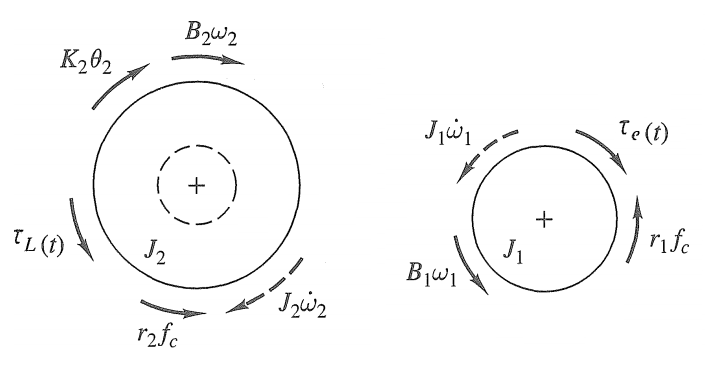
\includegraphics[width=0.5\linewidth]{Rotational_free-body}
	\caption{Rotational mechanical free-body diagram.}
	\label{fig:rotational_free-body}
\end{figure}
where $\theta$ is the angular displacement, $\omega$ is the angular speed, $B$ is the rotational viscous-damping coefficient, $K$ is the stiffness coefficient, $J$ is the moment of inertia, $f_c$ is the contact force between two gears, and $r$ is the gear radius.

The electromechanical section (DC motor) is

\begin{figure}[H]
	\centering
	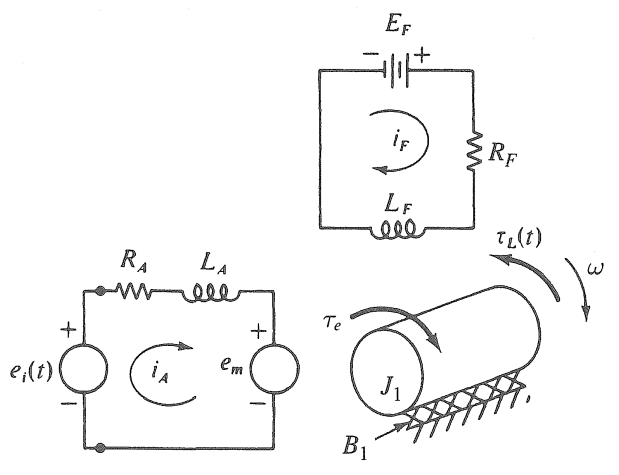
\includegraphics[width=0.5\linewidth]{Electromechanical_free-body}
	\caption{Electromechanical free-body diagram.}
	\label{fig:electromechanical_free-body}
\end{figure}
where $R_F$ is the field resistance, $L_F$ is the field inductance, $E_F$ is the applied constant field voltage, and $i_F$ is the input field current. $R_A$ is the stationary resistance, $L_A$ is the stationary inductance, and $e_m$ is the induced voltage, $i_A$ is the input stationary current, and $e_i(t)$ is the applied armature voltage, and $\tau_e$ is the electromechanical driving torque exerted on the rotor. 

If the flux density $\mathcal{B}$ is
\begin{align}
	\mathcal{B} & = \frac{\phi(i_F)}{A}           \\
	\intertext{the torque on the rotor is}
	\tau_e      & = \mathcal{B} l a~i_A \nonumber \\
	\tau_e      & = \frac{l a}{A} \phi(i_F) i_A \label{eq:tau_e}
\end{align}
where $\phi(i_F)$ is the flux induced by $i_F$, $A$ is the cross-sectional area of the flux path in the air gap between the rotor and stator, $l$ is the total length of the armature conductors within the magnetic field, and $a$ is the radius of the armature.

Also, the voltage induced in the armature $e_m$ can be written as
\begin{align}
	e_m & = \frac{l a}{A} \phi(i_F) \omega
\end{align}
where both, $\tau_e$ and $e_m$, depend on the geometry of the DC motor. 


\section{Dynamic system}
We begin applying D'Alembert's law (restatement of Newton's law) to the rotational mechanical section.
\begin{align}
	\sum \tau_{all}                                          & = 0 \nonumber                 \\
	J_1 \dot{\omega}_1 + B_1 \omega_1 + r_1 f_c              & = \tau_e(t)   \label{eq:Rot1} \\
	J_2 \dot{\omega}_2 + B_2 \omega_2 + K_2 \theta - r_2 f_c & = \tau_L(t)	 \label{eq:Rot2}
\end{align}
where $\tau_{all}$ are the torques acting on a body, $K\theta$ is the stiffness torque, $B\omega$ is the viscous-frictional torque, $J\dot{\omega}$ is the inertial torque, $\tau_e(t)$ is the driving torque,  $\tau_L(t)$ is the load torque, and $r f_c$ is the contact torque.

Due to the relation between gears,
\begin{align*}
	\theta_1       & = N \theta_2       \\
	\omega_1       & = N \omega_2       \\
	\dot{\omega}_1 & = N \dot{\omega}_2 \\
	N              & = \frac{r_2}{r_1}
\end{align*}
where $N$ is the gear radius relation. We solve \eqref{eq:Rot1} and \eqref{eq:Rot2} in terms of $\omega_2$ and $\theta_2$,
\begin{align}
	(J_2+N^2 J_1)\dot{\omega}_2+(B_2+N^2 B_1)\omega_1+K_2 \theta_2-N \tau_e(t)-\tau_L(t) = 0 \nonumber 
\end{align}
defining the relations
\begin{align*}
	J_{eq} & = J_2+N^2 J_1 \\
	B_{eq} & = B_2+B^2 B_1
\end{align*}
it becomes in
\begin{align}	
	J_{eq} \dot{\omega}_2+B_{eq} \omega_2+K_2 \theta_2-N \tau_e(t)-\tau_L(t) = 0 \label{eq:Rot3}
\end{align}

Now, let us derive the equations of the electromechanical section using Kirchoff's law.
\begin{align}
	\sum V_{all}            & = 0 		\nonumber             \\
	e_m+V_{L_{A}}+V_{R_{A}} & = e_i(t) 	\label{eq:Elec1}
\end{align}
where $V_{all}$ are the induced voltages on the rotor and stator, $V_{L_{A}}$ is the stationary resistance voltage, $V_{R_{A}}$ is the stationary inductance voltage.  

If $i_F$ is defined as constant, then \eqref{eq:tau_e} is
\begin{align}
	\tau_e(t) & = \left( \frac{l a}{A} \phi(i_F) \right) i_A(t)	\nonumber \\
	\tau_e(t) & = \alpha i_A(t)
\end{align}
where $\alpha$ is the internal parameters of the DC motor.

Then, simplifying and using \eqref{eq:Rot3} and \eqref{eq:Elec1} the dynamic system is, 
\begin{align}
	J_{eq} \dot{\omega}_2+B_{eq} \omega_2+K_2 \theta_2-N \tau_e - \tau_L & = 0 \\
	L_A \dot{i}_A + R_A i_A + \alpha \omega_1 - e_i                      & = 0
\end{align}

\section{State-space equations}
Let us define the state-space equations for $x=\left[ \theta_2~\dot{\theta}_2~i_A \right]^{\intercal}$. From the dynamic system,
\begin{align*}
	J_{eq} \ddot{\theta}_2+B_{eq} \dot{\theta}_2+K_2 \theta_2-N \alpha i_A-\tau_L & = 0 \\
	L_A \dot{i}_A + R_A i_A + \alpha \omega_1 - e_i                               & = 0                              
\end{align*}
reordering,
\begin{align*}
	\ddot{\theta}_2 & = -\frac{B_{eq}}{J_{eq}} \dot{\theta}_2 - \frac{K_2}{J_{eq}} \theta_2 + \frac{N \alpha}{J_{eq}} i_A - \frac{1}{J_{eq}} \tau_L \\
	\dot{i}_A       & = -\frac{R_A}{L_A} i_A -\frac{N \alpha}{L_A} \dot{\theta}_2 + \frac{1}{L_A} e_i
\end{align*}
defining the states as
\begin{align*}
	\begin{cases}
		x_1 & = \theta_2, \quad \dot{x}_1 = \dot{\theta}_2 = x_2                                                                                                                                   \\
		x_2 & = \dot{\theta}_2, \quad \dot{x}_2  = \ddot{\theta}_2 =  -\frac{B_{eq}}{J_{eq}} x_2 - \frac{K_2}{J_{eq}} x_1 + \frac{N \alpha}{J_{eq}} x_3 - \frac{1}{J_{eq}} \tau_L \\
		x_3 & = i_A, \quad \dot{x}_3 = \dot{i}_A = -\frac{R_A}{L_A} x_3 -\frac{N \alpha}{L_A} x_2 + \frac{1}{L_A} e_i
	\end{cases}	
\end{align*}
then
\begin{align}
\begin{bmatrix}
	\dot{x}_1 \\
	\dot{x}_2 \\
	\dot{x}_3
\end{bmatrix}
&=
\underbrace{
	\begin{bmatrix}
		0                   & 1                      & 0                       \\
		-\frac{K_2}{J_{eq}} & -\frac{B_{eq}}{J_{eq}} & \frac{N \alpha}{J_{eq}} \\
		0                   & -\frac{N \alpha}{L_A}  & -\frac{R_A}{L_A}
	\end{bmatrix}
}_A
\underbrace{
	\begin{bmatrix}
		x_1 \\
		x_2 \\
		x_3
	\end{bmatrix}
}_\mathbf{x}
+
\underbrace{
	\begin{bmatrix}
		0 & 0               & 0             \\
		0 & -\frac{1}{J_eq} & 0             \\
		0 & 0               & \frac{1}{L_A}
	\end{bmatrix}
}_B
\underbrace{
	\begin{bmatrix}
		0      \\
		\tau_L \\
		e_i
	\end{bmatrix}
}_\mathbf{u}
\\
\mathbf{\dot{x}} &= A \mathbf{x} + B \mathbf{u} \label{eq:sys1}
\end{align}

The output $y=\dot{\omega}_2$ can be defined as
\begin{align}
y &=
\underbrace{
	\begin{bmatrix}
		0 & 1 & 0
	\end{bmatrix}
}_C
\begin{bmatrix}
	x_1 \\
	x_2 \\
	x_3
\end{bmatrix}
+
\underbrace{
	\begin{bmatrix}
		0 & 0 & 0
	\end{bmatrix}
}_D
e_i
\\
y &= C \mathbf{\dot{x}}
\end{align}


\section{Equilibrium point $\mathbf{x_0}$}
Using $\mathbf{\dot{x}}=0$ in \eqref{eq:sys1}, the equilibrium point $\mathbf{x_0}$ can be calculated as 
\begin{align}
	0            & = A \mathbf{x_0} +B \mathbf{u} \\
	\mathbf{x_0} & = - A^{-1} B \mathbf{u} \\
	\begin{bmatrix}
		x_{1_0} \\
		x_{2_0} \\
		x_{3_0}
	\end{bmatrix}
	& = - 
	\begin{bmatrix}
		0                   & 1                      & 0                       \\
		-\frac{K_2}{J_{eq}} & -\frac{B_{eq}}{J_{eq}} & \frac{N \alpha}{J_{eq}} \\
		0                   & -\frac{N \alpha}{L_A}  & -\frac{R_A}{L_A}
	\end{bmatrix}^{-1}
	\begin{bmatrix}
		0 & 0               & 0             \\
		0 & -\frac{1}{J_eq} & 0             \\
		0 & 0               & \frac{1}{L_A}
	\end{bmatrix}
	\begin{bmatrix}
		0      \\
		\tau_L \\
		e_i
	\end{bmatrix}
\end{align}
Solving for no external torque $\tau_L=0$, constant applied armatrue voltage $e_i=E_0$, and $K_2 \neq 0$,
\begin{align*}
	0 & = x_{2_0}                                                                                      \\
	0 & = -\frac{K_2}{J_{eq}} x_{1_0} -\frac{B_{eq}}{J_{eq}} x_{2_0} + \frac{N \alpha}{J_{eq}} x_{3_0} \\
	0 & = -\frac{N \alpha}{L_A}  x_{2_0} -\frac{R_A}{L_A} x_{3_0} + \frac{1}{L_A} E_0
\end{align*}
due to $x_{2_0}=0$, we have
\begin{align*}
	0 & = -\frac{K_2}{J_{eq}} x_{1_0} + \frac{N \alpha}{J_{eq}} x_{3_0} \\
	0 & = -\frac{R_A}{L_A} x_{3_0} + \frac{1}{L_A} E_0
\end{align*}
then
\begin{align*}
	x_{1_0} & = \frac{N \alpha}{K_2 R_A} E_0 \\
	x_{3_0} & = \frac{1}{R_A} E_0
\end{align*}
therefore the equilibrium point is
\begin{align}
	\mathbf{x_0} &= 
	\begin{bmatrix}
		x_{1_0} \\
		x_{2_0} \\
		x_{3_0}
	\end{bmatrix}
	=
	\begin{bmatrix}
		\frac{N \alpha}{K_2 R_A} \\
		0 \\
		\frac{1}{R_A}
	\end{bmatrix}
	E_0
\end{align}

This equilibrium point indicates that a \textbf{constant angular displacement (twist)} produced by $x_{1_0}=\theta_{2_0}$ is sufficient to balance the constant applied armature voltage $e_i=E_0$.

On the other hand, if we solve for no external torque $\tau_L=0$, constant applied armature voltage $e_i=E_0$, and no stiffness $K_2 = 0$. The problem is,
\begin{align*}
	\begin{bmatrix}
		x_{1_0} \\
		x_{2_0} \\
		x_{3_0}
	\end{bmatrix}
	& = - 
	\begin{bmatrix}
		0 & 1                      & 0                       \\
		0 & -\frac{B_{eq}}{J_{eq}} & \frac{N \alpha}{J_{eq}} \\
		0 & -\frac{N \alpha}{L_A}  & -\frac{R_A}{L_A}
	\end{bmatrix}^{-1}
	\begin{bmatrix}
		0 & 0               & 0             \\
		0 & -\frac{1}{J_eq} & 0             \\
		0 & 0               & \frac{1}{L_A}
	\end{bmatrix}
	\begin{bmatrix}
		0   \\
		0   \\
		E_0
	\end{bmatrix}
\end{align*}
if we eliminate $x_{1_0}$ because the first column of $A^{-1}$ has zeros, the problem reduces to
\begin{align}
	\begin{bmatrix}
		x_{2_0} \\
		x_{3_0}
	\end{bmatrix}
	& = - 
	\begin{bmatrix}
		-\frac{B_{eq}}{J_{eq}} & \frac{N \alpha}{J_{eq}} \\
		-\frac{N \alpha}{L_A}  & -\frac{R_A}{L_A}
	\end{bmatrix}^{-1}
	\begin{bmatrix}
		-\frac{1}{J_eq} & 0             \\
		0               & \frac{1}{L_A}
	\end{bmatrix}
	\begin{bmatrix}
		0   \\
		E_0
	\end{bmatrix}
\end{align}
solving, we have
\begin{align}
	\begin{bmatrix}
		x_{2_0} \\
		x_{3_0}
	\end{bmatrix}
	& = 
	\begin{bmatrix}
		\frac{N \alpha}{B_{eq} R_A+(N \alpha)^2}\\
		\frac{-B_{eq}}{B_{eq} R_A+(N \alpha)^2}
	\end{bmatrix}
	E_0
\end{align}
which indicates that a \textbf{constant angular speed} produced by $x_{2_0}=\dot{\theta_{2_0}}$ is needed to balance the constant applied armature voltage $e_i=E_0$.




\begin{thebibliography}{99}
	\bibitem{close} Close, Charles M. and Frederick, Dean K. and Newell, Jonathan C., \textit{Modeling and Analysis of Dynamic Systems}, 2001, ISBN 0471394424.
\end{thebibliography}




\end{document}
